
\documentclass[border=10pt]{standalone}

\usepackage[utf8]{inputenc}                                 % Codificação do documento
\usepackage[T1]{fontenc}                                    % Seleção de código de fonte
\usepackage{microtype}                                      % Melhora a justificação do documento
\usepackage{lmodern}                                       % Usa a fonte Latin Modern
\usepackage{ae, aecompl}                                    % Fontes de alta qualidade

\usepackage{amsmath}
\usepackage{verbatim}
\usepackage{tikz}
\usetikzlibrary{calc,positioning,shadows.blur,decorations.pathreplacing}
\usepackage{etoolbox}

\tikzset{
        label/.style = { black, midway, scale=0.5, align=center },
     toplabel/.style = { label, above=.5em, anchor=south },
    leftlabel/.style = { label,rotate=-90,left=.5em,anchor=north },
  bottomlabel/.style = { label, below=.5em, anchor=north },
        force/.style = { rotate=-90,scale=0.4 },
        round/.style = { rounded corners=2mm },
       legend/.style = { right,scale=0.6 },
        nosep/.style = { inner sep=0pt },
   generation/.style = { anchor=base,scale=0.6 }
}

\begin{document}
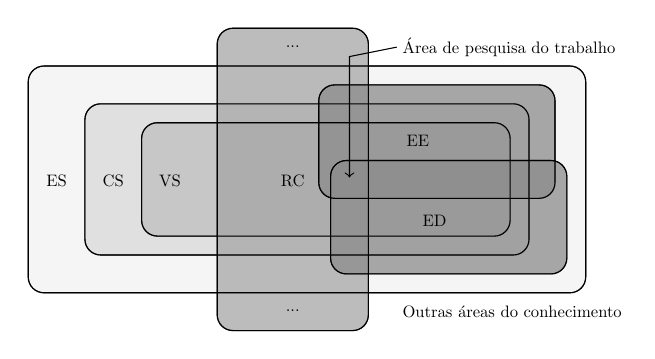
\begin{tikzpicture}[x=1.2cm, y=1.2cm]
  % retangules
  \draw[round,fill=black!5, opacity=0.75] (-0.7,-0.1) rectangle (5.2,-2.5);
  \draw[round,fill=black!15,opacity=0.75] (-0.1,-0.5) rectangle (4.6,-2.1);
  \draw[round,fill=black!25,opacity=0.75] (0.5,-0.7) rectangle (4.4,-1.9);

  \draw[round,fill=black!35,opacity=0.75] (1.3,0.3) rectangle (2.9,-2.9);

  \draw[round,fill=black!45,opacity=0.75] (2.375,-0.3) rectangle (4.875,-1.5);
  \draw[round,fill=black!45,opacity=0.75] (2.5,-1.1) rectangle (5.0,-2.3);

  % outlines
  \draw[round,fill=none] (-0.7,-0.1) rectangle (5.2,-2.5);
  \draw[round,fill=none] (-0.1,-0.5) rectangle (4.6,-2.1);
  \draw[round,fill=none] (0.5,-0.7) rectangle (4.4,-1.9);

  \draw[round,fill=none] (1.3,0.3) rectangle (2.9,-2.9);

  \draw[round,fill=none] (2.375,-0.3) rectangle (4.875,-1.5);
  \draw[round,fill=none] (2.5,-1.1) rectangle (5.0,-2.3);

  \node at(-0.4,-1.37) [generation] {ES};
  \node at(0.2,-1.37) [generation] {CS};
  \node at(0.8,-1.37) [generation] {VS};

  \node at(2.1,-1.37) [generation] {RC};
  \node at(2.1, 0.1) [generation] {...};
  \node at(2.1,-2.7) [generation] {...};

  \node at(3.425,-0.95) [generation] {EE};
  \node at(3.6,-1.8) [generation] {ED};

  % \node at(3.65,-1.37) [generation] {EDS \& EES};

  \draw [<-] (2.7,-1.28)  --  (2.7,0.0)  --  (3.2,0.1) node [legend] {Área de pesquisa do trabalho};
  \node at(3.2,-2.7) [legend] {Outras áreas do conhecimento};

  %\node at(4.25,-0.5) [force]      {strong nuclear force (color)};
  %\node at(4.85,-1.5) [force]    {electromagnetic force (charge)};
  %\node at(5.45,-2.4) [force] {weak nuclear force (weak isospin)};
  %\node at(6.75,-2.5) [force]        {gravitational force (mass)};

  %
  %\draw [<-] (2.5,0.15)  -- (2.7,0.15)         node [legend] {colors};
  %\draw [<-] (2.05,0.25) -- (2.3,0) -- (2.7,0) node [legend]   {mass};
  %\draw [<-] (2.5,-0.3)  -- (2.7,-0.3)         node [legend]   {spin};

  %\node at (0,1.2)   [generation] {1\tiny st};
  %\node at (1,1.2)   [generation] {2\tiny nd};
  %\node at (2,1.2)   [generation] {3\tiny rd};
  %\node at (2.8,1.2) [generation] {\tiny generation};
\end{tikzpicture}
\end{document}
